%!TEX root = ../../csuthesis_main.tex

\subsection{基于TSAVN的多无人机任务调度分配算法设计} \label{sec:TSAVN}

K-Means算法是一种机器学习中常用的聚类算法,其认为样本间距离越近,则这两个样本的相似性越大。其时间复杂度仅为\(tknm\),其中\(t\)为迭代次数,\(k\)为类别簇的个数,\(n\)为样本个数,\(m\)为样本的纬度,能够在很短时间内将\(n\)个样本根据欧式距离计算样本间的相似度,无需对样本进行任何标注,即可将其聚类分为\(k\)个类别。

模拟退火算法(Simulated Annealing Algorithm, SA)是一种模拟热力学中退火的过程,从某一较高的初始温度开始,随着算法迭代次数的增加而逐渐降低温度,结合概率跳跃的特性使得算法在温度高时具备跳出当前所在的局部最优解,在解的邻域结构中随机搜索全局最优解的启发式算法。

变邻域搜索算法(Varied Neighborhood Search Algorithm, VNS)是一种改进型的局部搜索算法,其利用了全局最优解必然在任意邻域结构中仍为局部最优解的特点,利用不同邻域动作所构成的邻域结构进行交替搜索,拓展了解的搜索范围,在集中性与疏散性之间达到了较好的平衡。

\subsubsection{算法设计} 

多无人机任务调度分配算法将分为两个阶段,分别是对任务进行预分配的预分配阶段,以及基于预分配的任务信息,得到无人机所需数量及各无人机的任务有序序列的再分配阶段,如图~\ref{fig:多无人机任务调度分配阶段示意图}所示,其中,在任务预分配阶段,由于对于无人机而言,若执行相邻任务距离较远,且跨过了数个其他任务点,那么其最终的航程通常较大,而执行相邻任务距离较远,且中途没有其他任务点,那么其最终的航程通常较小,因此可以通过对任务点间的飞行航迹的航程进行聚类来得到初步的任务预分配结果,是合理的;之后,由于任务预分配结果仅仅只是根据航程信息对任务进行聚类操作,不具备问题所需的无人机数量、各无人机所要执行的任务有序序列,因此在任务再分配阶段,本文提出了TSAVN算法,其流程图如图~\ref{fig:多无人机任务调度分配阶段示意图}所示。

\begin{figure}[!htbp]
    \centering
    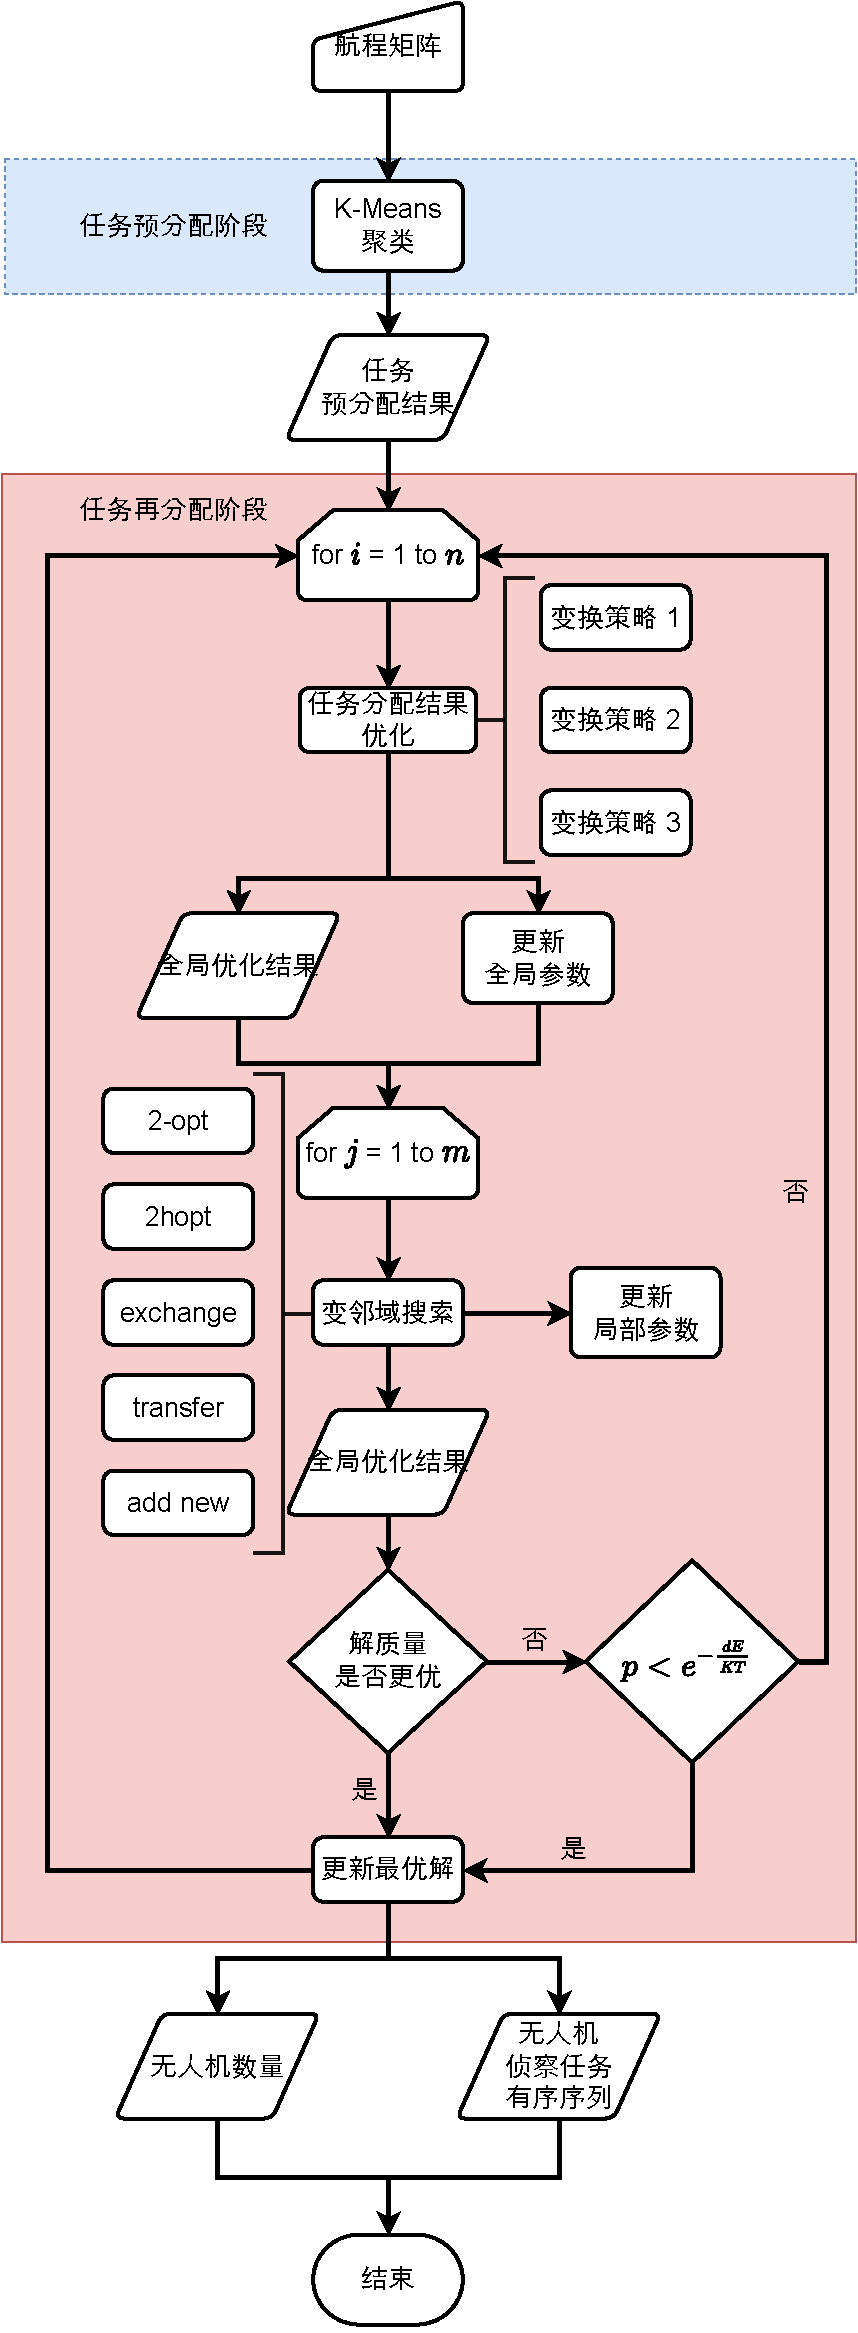
\includegraphics[width=0.55\textwidth]{images/多无人机任务调度分配阶段示意图.pdf}
    \caption{多无人机任务调度分配阶段示意图}
    \label{fig:多无人机任务调度分配阶段示意图}
\end{figure}

由于直接使用任务点数据会导致解空间过大的问题,故先使用K-Means算法根据点间的航程数据,对任务点数据进行聚类,使得各个类内距离尽可能近,类间距离尽可能远,实现任务的预分配,从而能够有效地降低各个部分的解空间,便于并行、高效地运行算法。

本小节以最小化航迹距离作为聚类依据,自下而上对各任务点进行聚类。同时为尽可能保证同一个簇里航迹之和最小,在聚类完成后,将结果放入局部优化器中生成各个簇中最优的车辆安排、配置及路径等数据,即初始解生成。

初始解生成的伪代码如算法\ref{alg:Solution Initialization}所示:

\begin{algorithm}[!htbp]
  \caption{初始解生成器} % 名称
  \label{alg:Solution Initialization}
  \begin{algorithmic}[1]
    \REQUIRE 
      \( V \): 无人机起飞点与任务点的点集;
      \( M \): 所有任务点的任务数据集;
      \( C \): 所有车型数据集;
    \ENSURE 
      \( S \): 初始解;
    \STATE 初始化类簇标签 \( L \);
    \REPEAT
        \STATE 获取距离矩阵 \(D \gets \textrm{CalcDistanceMatrix}(V, L) \);
        \STATE 获取所有拥有最小距离的两个簇的组合 \(C \gets \textrm{FindMinDisCombs}(L, D) \);
        \FOR{\( i, j \in C \)}
            \IF{\( \textrm{not} \textrm{ReachCriteria}(i, j, L) \)}
                \STATE 更新标签 \( L \gets \textrm{merge}(i, j, L) \);
            \ENDIF
        \ENDFOR
    \UNTIL {\( \textrm{AllReachCriteria}(L) \)}
    \STATE \( S \gets \textrm{PartialSolver}(L, V, M, C) \);
  \end{algorithmic}
\end{algorithm}

为了增加算法收敛至全局最优解的概率,以及尽可能避免算法生成的解质量较差的情况发生,本小节选取了3种不同的解的变化策略,以及5种基于这3种方式的邻域结构来对全局解中不同任务簇的分类进行一定的调整。

第一种变化策略为任务点的转移,将一个簇中的任务点转移至另一个簇中,过程如图\ref{fig:conversion_way_1}所示。基于该变化策略,本文提出了两种随机性不同的邻域结构。一种在两个簇中的选取及待转移的任务点的选取中全部依赖随机,即随机性较高,其动作过程的伪代码如算法\ref{alg:Stochastic Transfer Neighborhood Structure}所示;另一种则随机选取一个簇并随机选取簇中的一个任务点,将其转移至离该簇最近的另一个簇中,随机性相对于前者更低,但相应的计算时间更多,其动作过程的伪代码如算法\ref{alg:Proximity Transfer Neighborhood Structure}所示。

\begin{figure}[!htbp]
    \centering
    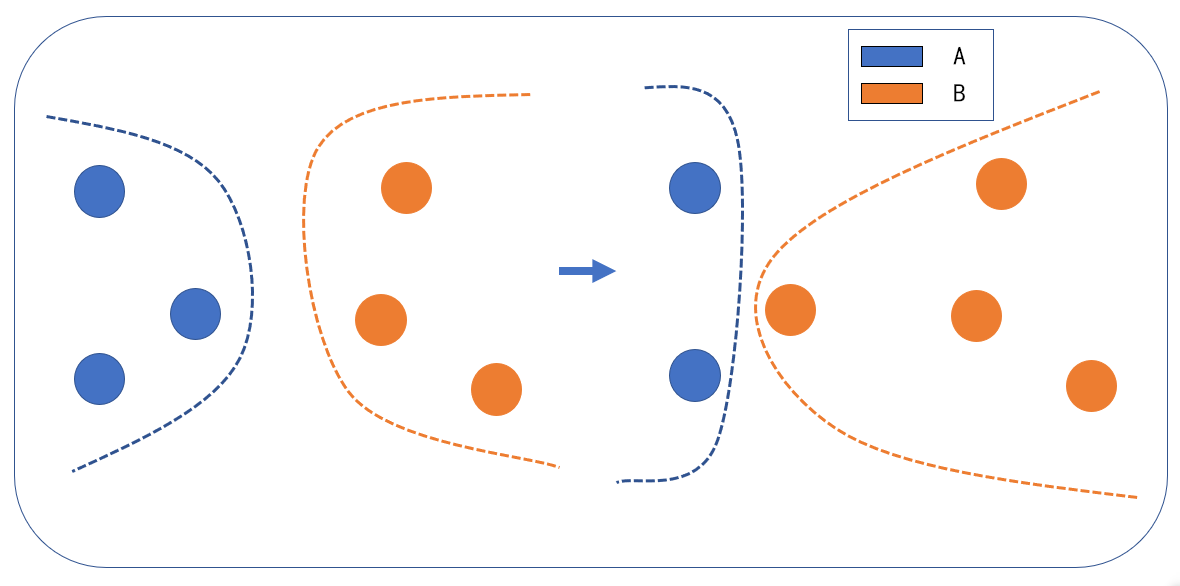
\includegraphics[width=0.7\textwidth]{images/全局邻域1_en.png}
    \caption{变化策略 1}
    \label{fig:conversion_way_1}
\end{figure}

\begin{algorithm}[!htbp]
  \caption{随机转移算子} % 名称
  \label{alg:Stochastic Transfer Neighborhood Structure}
  \begin{algorithmic}[1]
    \REQUIRE
      $V$: 无人机起飞点与任务点的点集;
      $L$: 先前的类簇标签;
    \ENSURE
      $L^*$: 新的类簇标签;
    \STATE 随机寻找两个类簇 $\ell_1, \ell_2 \gets$ FindTwoDifferentLabel($L$);
    \STATE 在类簇$\ell_1$中寻找一个随机的任务点$v_1$;
    \STATE 更新任务点 $v_1$'的标签从 $\ell_1$ 变为 $\ell_2$;
    \STATE $L^* \gets L$;
  \end{algorithmic}
\end{algorithm}

\begin{algorithm}[!htbp]
  \caption{就近转移算子} % 名称
  \label{alg:Proximity Transfer Neighborhood Structure}
  \begin{algorithmic}[1]
    \REQUIRE
      $V$: 无人机起飞点与任务点的点集;
      $L$: 先前的类簇标签;
    \ENSURE
      $L^*$: 新的类簇标签;
    \STATE 随机寻找一个类簇 $\ell_1 \gets$ FindLabel($L$);
    \STATE 寻找一个距离$\ell_1$最近的类簇 $\ell_2 \gets$ FindNearestLabel($L, \ell_1$);
    \STATE 在类簇$\ell_1$中寻找一个随机的任务点$v_1$;
    \STATE 更新任务点 $v_1$'的标签从 $\ell_1$ 变为 $\ell_2$;
    \STATE $L^* \gets L$;
  \end{algorithmic}
\end{algorithm}

第二种变化策略为任务点的交换,在两个不同的簇中各自选择一个任务点进行交换,其过程如算法\ref{fig:conversion_way_2}所示。基于该变化策略,本文提出了两种随机性不同的邻域结构,一种在两个簇的选取及各自的待交换的任务点的选取中全部依赖随机,即随机性较高,其动作过程的伪代码如算法\ref{alg:Stochastic Exchange Neighborhood Structure}所示;另一种则随机选取一个簇,并将离它最近的簇作为另一个簇,分别随机选取簇中的任务点进行交换,随机性相对于前者更低,但相应的计算时间会更多,其动作过程的伪代码如算法\ref{alg:Proximity Exchange Neighborhood Structure}所示。

\begin{figure}[!htbp]
    \centering
    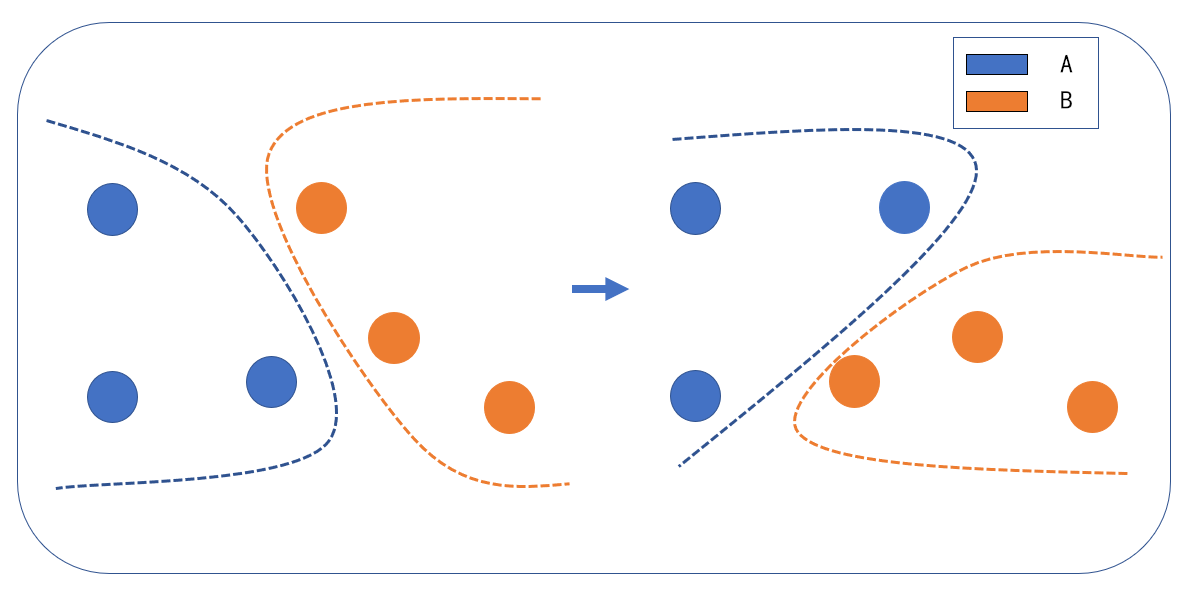
\includegraphics[width=0.7\textwidth]{images/全局邻域2_en.png}
    \caption{变化策略 2}
    \label{fig:conversion_way_2}
\end{figure}

\begin{algorithm}[!htbp]
  \caption{随机交换算子} % 名称
  \label{alg:Stochastic Exchange Neighborhood Structure}
  \begin{algorithmic}[1]
    \REQUIRE
      $V$: 无人机起飞点与任务点的点集;
      $L$: 先前的类簇标签;
    \ENSURE
      $L^*$: 新的类簇标签;
    \STATE 随机寻找两个类簇 $\ell_1, \ell_2 \gets$ FindTwoDifferentLabel($L$);
    \STATE 在类簇$\ell_1$中寻找一个随机的任务点$v_1$;
    \STATE 在类簇$\ell_2$中寻找一个随机的任务点$v_2$;
    \STATE 更新任务点 $v_1$'的标签从 $\ell_1$ 变为 $\ell_2$;
    \STATE 更新任务点 $v_2$'的标签从 $\ell_2$ 变为 $\ell_1$;
    \STATE $L^* \gets L$;
  \end{algorithmic}
\end{algorithm}

\begin{algorithm}[!htbp]
  \caption{就近交换算子} % 名称
  \label{alg:Proximity Exchange Neighborhood Structure}
  \begin{algorithmic}[1]
    \REQUIRE
      $V$: 无人机起飞点与任务点的点集;
      $L$: 先前的类簇标签;
    \ENSURE
      $L^*$: 新的类簇标签;
    \STATE 随机寻找一个类簇 $\ell_1 \gets$ FindLabel($L$);
    \STATE 寻找一个距离$\ell_1$最近的类簇 $\ell_2 \gets$ FindNearestLabel($L, \ell_1$);
    \STATE 在类簇$\ell_1$中寻找一个随机的任务点$v_1$;
    \STATE 在类簇$\ell_2$中寻找一个随机的任务点$v_2$;
    \STATE 更新任务点 $v_1$'的标签从 $\ell_1$ 变为 $\ell_2$;
    \STATE 更新任务点 $v_2$'的标签从 $\ell_2$ 变为 $\ell_1$;
    \STATE $L^* \gets L$;
  \end{algorithmic}
\end{algorithm}

第三种变化策略则是生成新的簇,选取一个任务点作为一个新的类,其过程如算法\ref{fig:Conversion_Way_3}所示。基于该变化策略,本文提出了一种邻域结构,该邻域结构为随机选取一个任务点,若该任务点所属的簇包含的任务点不止该任务点,则将该任务点作为一个新的簇,其动作过程的伪代码如算法\ref{alg:New Cluster Generation Neighborhood Structure}所示;

\begin{figure}[!htbp]
    \centering
    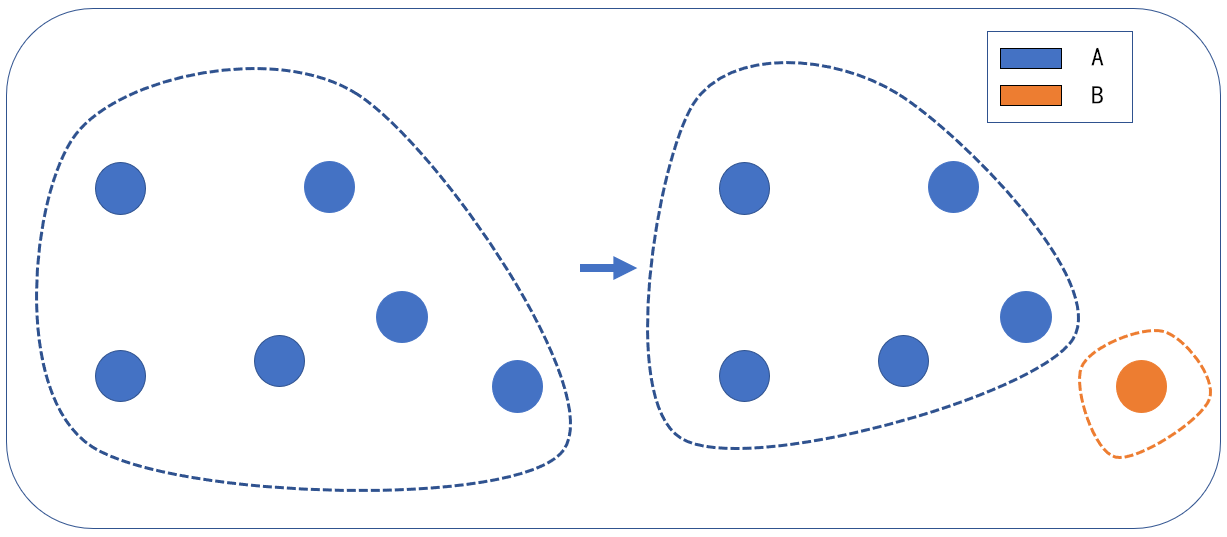
\includegraphics[width=0.7\textwidth]{images/全局邻域3_en.png}
    \caption{变化策略 3}
    \label{fig:Conversion_Way_3}
\end{figure}

\begin{algorithm}[!htbp]
  \caption{新簇生成算子} % 名称
  \label{alg:New Cluster Generation Neighborhood Structure}
  \begin{algorithmic}[1]
    \REQUIRE
      $V$: 无人机起飞点与任务点的点集;
      $L$: 先前的类簇标签;
    \ENSURE
      $L^*$: 新的类簇标签;
    \STATE 随机寻找一个类簇 $\ell_1 \gets$ FindLabel($L$);
    \STATE 在类簇$\ell_1$中寻找一个随机的任务点$v_1$;
    \STATE 设置 $v_1$'的类簇标签为一个新的标签;
    \STATE $L^* \gets L$;
  \end{algorithmic}
\end{algorithm}

为了能够在每一个任务类簇中得到最优解,以获得全局的最优解,同时避免每个任务类簇中发生得到质量较差的解的情况,本小节选取了5种不同的邻域结构来对无人机的侦察任务执行序列进行调整和优化。

第一种邻域结构为2-opt方法\citep{croes1958MethodSolvingTravelingSalesman},如图~\ref{fig:2-opt邻域结构}所示。2-opt方法是选取两任务点\( i \)和\( k \),将\( i \)之前的任务序列保持不变,将\( k \)之后的任务序列保持不变,将\( i \)、\( k \)及其中间的任务的顺序进行翻转,来得到新的任务序列。

\begin{figure}[!htbp]
    \centering
    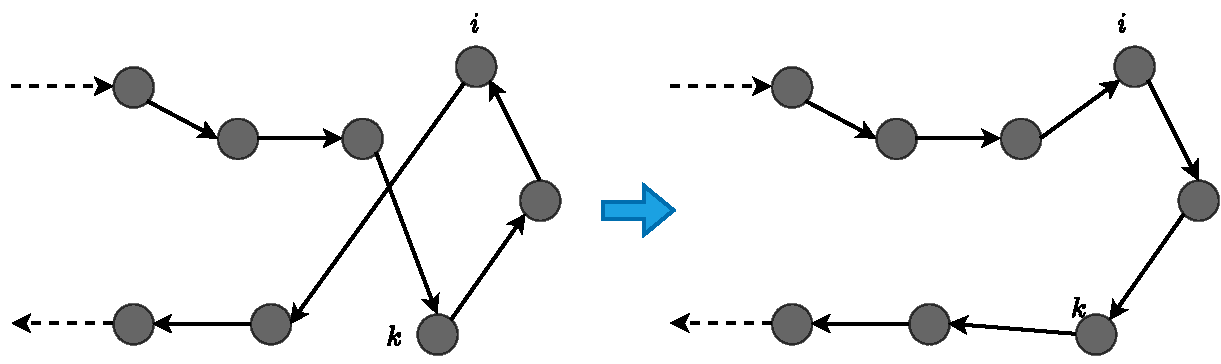
\includegraphics[width=0.8\textwidth]{images/2-opt.pdf}
    \caption{2-opt邻域结构}
    \label{fig:2-opt邻域结构}
\end{figure}

第二种邻域结构为2hopt方法,如图~\ref{fig:2hopt邻域结构}所示。2hopt方法是选取两任务点\( i \)和\( k \),将\( i \)之前的任务序列保持不变,将\( i \)与\( k \)之间的任务保持不变,将\( k \)之后的任务序列保持不变,仅将任务\( i \)、\( k \)进行交换,来得到新的任务序列。

\begin{figure}[!htbp]
    \centering
    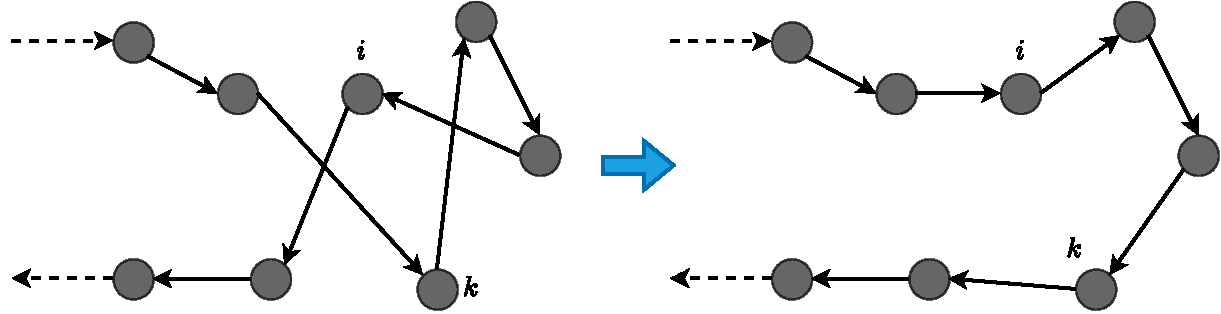
\includegraphics[width=0.8\textwidth]{images/2hopt.pdf}
    \caption{2hopt邻域结构}
    \label{fig:2hopt邻域结构}
\end{figure}

第三种邻域结构为exchange方法,如图~\ref{fig:exchange邻域结构}所示。exchange方法是对于两个无人机的任务序列而言,各选择其中的一个任务点\( i \)和\( k \),将任务点\( i \)和任务点\( k \)进行交换,其余任务点及序列保持不变,以此来得到两条新的任务序列。

\begin{figure}[!htbp]
    \centering
    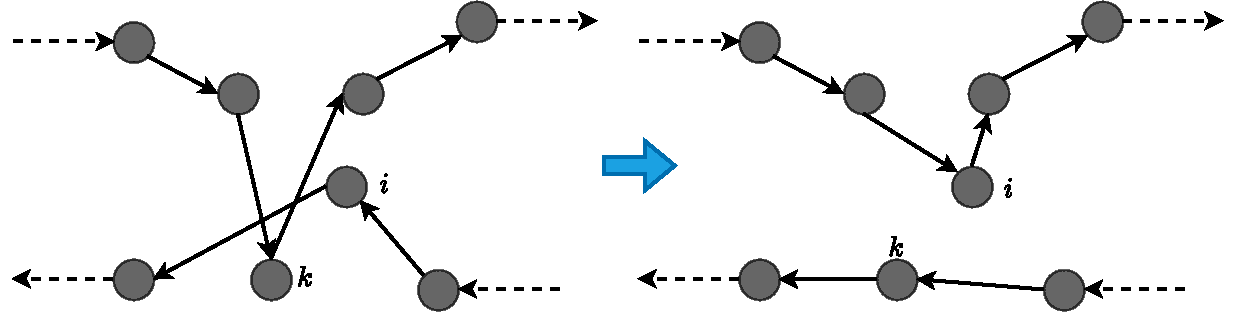
\includegraphics[width=0.8\textwidth]{images/exchange.pdf}
    \caption{exchange邻域结构}
    \label{fig:exchange邻域结构}
\end{figure}

第四种邻域结构为transfer方法,如图~\ref{fig:transfer邻域结构}所示。transfer方法是选取两任务点\( i \)和\( k \),将任务点\( i \)移出原任务序列,并将其插入至任务点\( k \)后,其余任务点及序列保持不变,以此来得到两条新的任务序列。

\begin{figure}[!htbp]
    \centering
    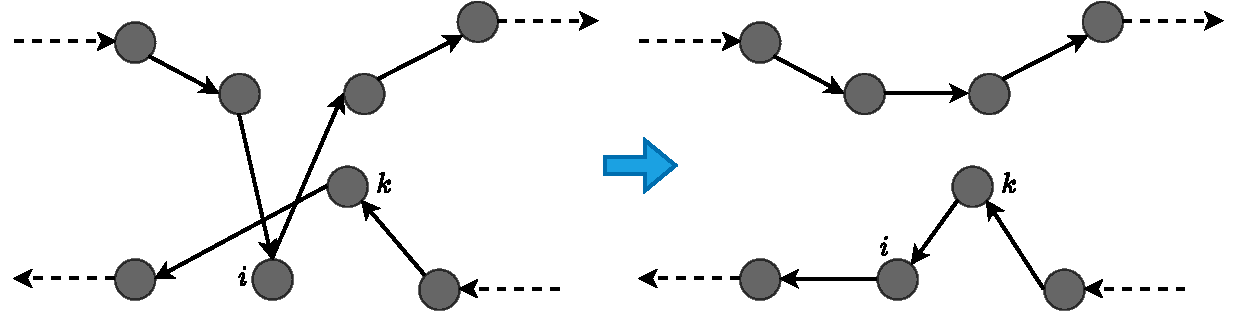
\includegraphics[width=0.8\textwidth]{images/transfer.pdf}
    \caption{transfer邻域结构}
    \label{fig:transfer邻域结构}
\end{figure}

第五种邻域结构为add new方法,如图~\ref{fig:add new邻域结构}所示。add new方法是选取一个任务点\( i \),将其从原任务序列中移除,其余任务点及序列保持不变,并将其作为新的无人机的任务序列,以此来得到两条新的任务序列。

\begin{figure}[!htbp]
    \centering
    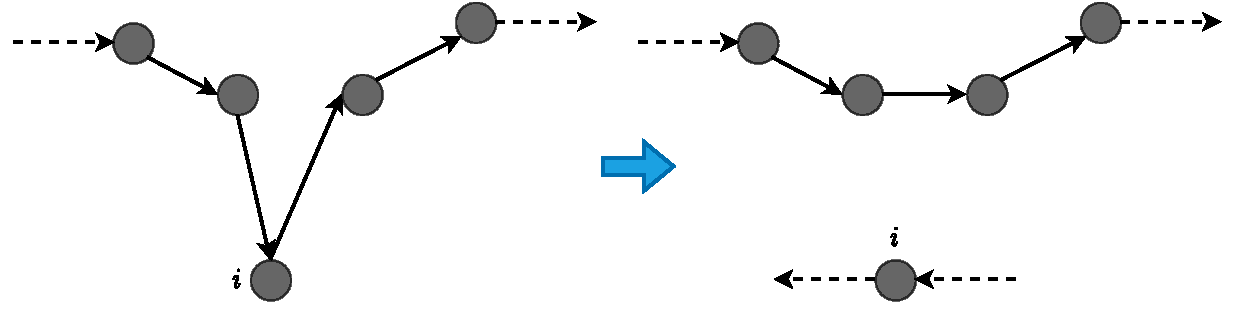
\includegraphics[width=0.8\textwidth]{images/add_new.pdf}
    \caption{add new邻域结构}
    \label{fig:add new邻域结构}
\end{figure}

由于模拟退火算法在运行中会存在初期温度高,同时未达到局部最优解的情况,以及末期温度低,同时达到局部最优解的情况,导致其非更优解接受概率的利用程度不高,所以模拟退火算法的性能仍有待提高。

为提高模拟退火算法的性能,更充分地利用其跳出局部最优解的机制,此处采用了自适应温度机制取代了原有的温度机制。

此处引入\(r_{i}\)作为算法第\(i\)次运行后没有得到更优解的次数,即需要计算非更优解接受概率的次数,当直接得到了更优解时\(r_{i} = 0\),算法未运行时\(r_{0} = 0\),即

\begin{equation}
    r_i = 
    \begin{aligned} 
    \begin{cases}
        r_{i-1} + 1 \quad &\text{if} \quad \Delta E > 0\\
        r_{i-1} &\text{if} \quad \Delta E = 0 \\
        0 &\text{if} \quad \Delta E <     0
    \end{cases}
    \end{aligned}
    \nonumber
\end{equation}

同时使用迭代次数\(N\)来控制整个算法的逻辑。与模拟退火算法相比,其总的求解次数仅由\(N\)决定,而模拟退火算法的总求解次数为\(N \cdot \log_{r}\frac{T_{0}}{T_{\text{end}}}\)。

设定一个最低温度\(T_{\min}\),升温速率\(\rho\)以及温控参数\(\delta\),使得第\(i\)次计算温度\(T_{i}\)时使用如下公式:

\begin{equation}
    T_i = T_{\min} + \rho \cdot \ln (1 + \frac{r_i}{\delta})
    \nonumber
\end{equation}

如此便能够在能够寻求到最优解的情况下维持低温,在到达局部最优解、需要到达新的局部最优解时能够通过升高温度来跳出局部最优解,从而使算法具有更好的鲁棒性。

\subsection{多无人机航迹规划及任务分配算法流程图}

由上述内容可知,本文提出的航迹规划及任务分配算法的流程如下,在任务开始前,服务器分别从贮存任务数据的数据库和地图信息的数据库中获取任务数据、地图数据,再将以上数据一齐输入进RRT*-Connect算法中,得到起飞点与任务点、任务点与任务点之间的无人机飞行航迹和飞行航程信息,将航程信息矩阵输入进K-Means算法中对任务进行预分配,再将任务的预分配结果、航程矩阵以及无人机的最大航程一齐输入进TSAVN算法中,便得到了完成任务所需的无人机数量以及每个无人机需完成的收集型侦察任务有序序列,再根据该序列从此前得到的点间飞行航迹中进行拼接得到各个无人机的飞行航迹,再将以上信息作为指令发送给无人机,由无人机完成所给任务。该算法的总流程如图~\ref{fig:航迹规划及任务分配流程图}所示。

\begin{figure}[!htbp]
    \centering
    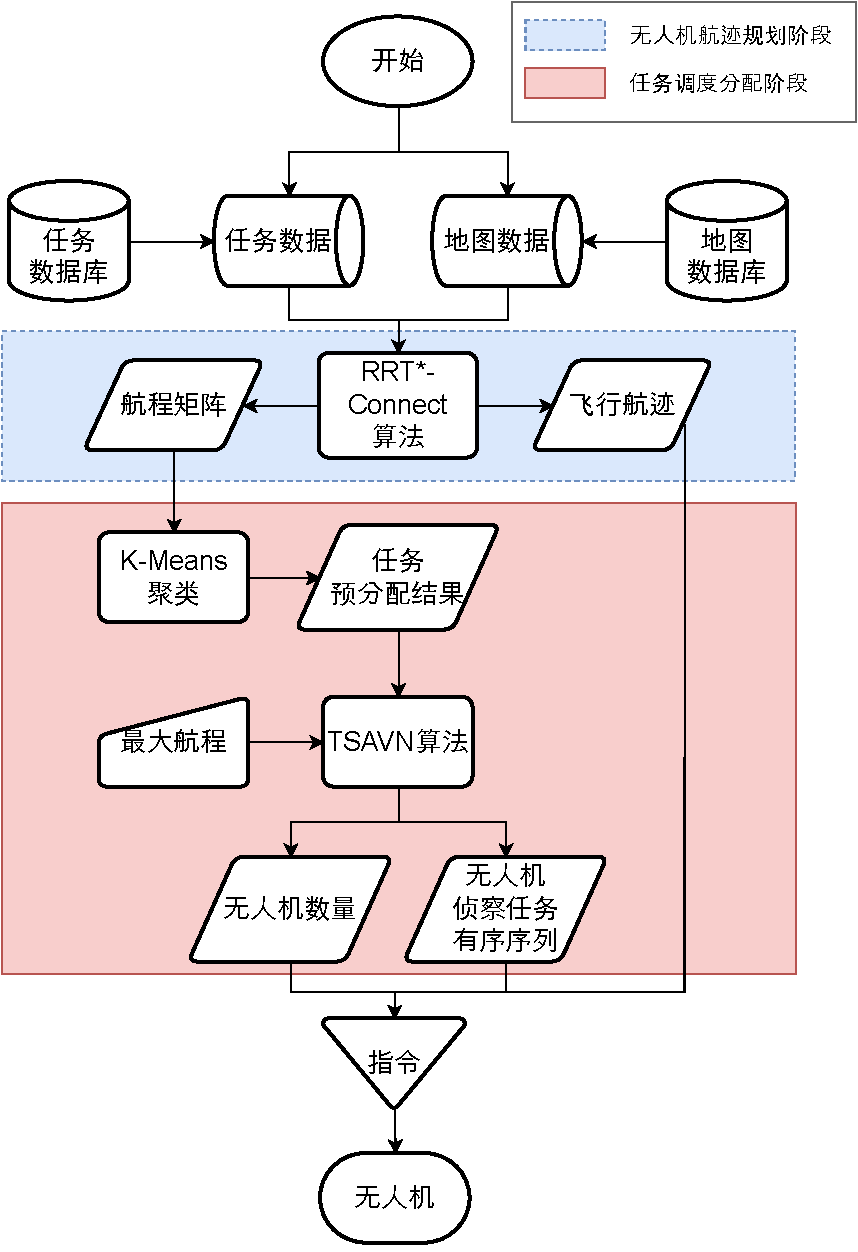
\includegraphics[width=0.7\textwidth]{images/任务分配及航迹规划算法流程图.drawio.pdf}
    \caption{航迹规划及任务分配流程图}
    \label{fig:航迹规划及任务分配流程图}
\end{figure}

\newpage
\section{本章小结}

本章主要对面向边缘计算的任务计算资源调度优化问题、多无人机的航迹规划及任务分配问题分别进行分析,并按照分析内容提出对应的求解算法,并详细说明了各个算法的关键机制、运行流程等内容。

\newpage
